\chapter{Social engineering} 
L'ingegneria sociale è la manipolazione psicologica delle persone per far si che eseguano azioni o divulghino informazioni personali. Sfrutta le vulnerabilità insite nelle persone.

Secondo Kevin Mitnick, uno degli hacker più famosi al mondo, anche se l'organizzazione investe pesantemente in sistemi di sicurezza, se l'attaccante riesce a fare quello che vuole anche a una sola persona, tutto l'investimento fatto è inutile.

Alcuni cyber criminali che usano l'ingegneria sociale sono:
\begin{itemize}
    \item Hacker: attacchi DDoS, ransomware, attacchi finanziari;
    \item Identity thieves: usano info che identificano la persona per i loro obiettivi (e poi possono rivenderle/pubblicarle online);
    \item Scam artists: eseguono azieni fraudolente o ingannevoli per frodare altri (es: lotteria scam su facebook).
\end{itemize}

\paragraph{Attacco alla banca del Bangladesh} Nel 2016 la banca del Bangladesh è stata vittima di una delle più grandi rapine informatiche. L'attacco è iniziato nel 2015, quando gli attaccanti sono riusciti ad installare un malware utilizzando un file malevolo spacciato per curriculum per una delle posizioni aperte nella banca. Lo scopo del malware era di eseguire una serie di trasferimenti verso una società no-profit estera. L'attacco è stato sventato dalla Federeal Reserve, dalla quale passano i trasferimenti internazionali, che si è accora dell'attacco grazie ad un errore di spelling nel nome dell'associazione.

\paragraph{Attacco a Macron} Caso di Identity Steal. Due francesi sono riusciti ad accedere alla mail di Macron, dalla quale hanno inviato mail che descrivevano i 10 motivi per cui non votare Macron.

\paragraph{Lotteria su Facebook} La persona viene contattata tramite Facebook informandola della vincita ad una lotteria e che l'assegno le verrà recapitato a casa. Alla consegna, alla vittima viene chiesto un pagamento per ricevere l'assegno.

\section{Ciclo di vita dell'attacco}
\begin{enumerate}
    \item Selezione del target;
    \item Reconnaissance;
    \item Raccolta delle info: posso cercare nella spazzatura della vittima ("dumpster diving" -> cerco bollette, stampe conto corrente, post-it con login e password, ...) o la osservo standone in prossimità ("shoulder surfing");
    \item Orchestrazione dell'attacco;
    \item Esecuzione dell'attacco: sfrutto le info e le relazioni per spingere la vittima a compiere le azioni che voglio;
    \item Impatto dell'attacco: raggiungo il mio obiettivo (es: installazione malware, eliminazione tracce attacco sulla macchina della vittima, ...).
\end{enumerate}

Possibili modi per ottenere informazioni: osservare alla spalle il target (es: mentre la persona sta lavorando al pc), cercare nella spazzatura del target.

\paragraph{Esempio di attacco}
\begin{itemize}
    \item  Obiettivo: ottenere dalla vittima le info necessarie ad eseguire un trasferimento di denaro;
    \item Selezione del target, reconnaissance, raccolte info: ad esempio verifico online se il target è stato vittima di attacchi di data breach;
    \item Attacck orchestration: ad esempio contatto la vittima tramite mail+telefono o sms+telefono;
    \item Esecuzione dell'attacco: 
	\begin{enumerate}
	    \item  Creo lo stage per l'attacco, creando ad esempio un sito web di phishing che simula il sito web di autenticazione della banca della vittima;
	    \item Creo un app malevola da far installare alla vittima, la quale mi girerà i codici ricevuti necessaria a superare l'autenticazione a più fattori;
	    \item Invio una mail alla vittima con il link alla pagina web;
	    \item  Contatto al vittima per telefono e la convinco a installare l'app. Per incrementare le possibilità di successo, posso camuffare il numero di telefono usando tecniche di spoofing facendo comparire il numero di telefono della banca;
	    \item  Se tutto ha successo, ottengo accesso all'home banking della vittima. 
	\end{enumerate}
    \item Impatto dell'attacco: Elimino ogni traccia dell'attacco (es: l'app si rimuove terminato il suo lavoro).
\end{itemize}

\section{Tipi di attacchi}
\begin{itemize}
    \item Phishing: condotto generalmente via mail, cerca di attaccare più persone possibili. Generalmente l'attaccante si finge una persona di alto rango o richiede che un'azione vengo svolta entro un breve limite di tempo;
    \item Spear phishing: mira ad una persona particolare;
    \item Whaling: mira a persone con elevate responsabilità nell'organizzazione;
    \item Viral hoaxe: mira a divulgare info false e quindi influenzare l'opinione delle persone. Sfrutta la curiosità delle persone (diffuso nei social, dove il post chiede di aprire il link per avere più info sull'argomento);
    \item Vhishing: usa chiamate telefoniche;
    \item Impersonation e tailgating: fatti di persona;
    \item SMiShing attacco tramite SMS.
\end{itemize}

\paragraph{Impersonation} Solitamente mi fingo qualcuno con autorità, qualcuno con seniority o un ente governativo.

\paragraph{Vishing} Un esempio di attacco è stato quello del falso servizio clienti di Apple. L'attaccante chiamava la vittima fingendosi il servizio clienti di Apple dicendo che c'era un problema con l'account Appl. Quando la vittima richiamava per risolvere, l'attaccante chiedeva i dati di accesso dell'account.

\paragraph{Tailgating} Sfrutta l'indole delle persone ad aiutare gli altri (es: mi fingo un dipendente della banca che ha dimenticato il tesserino di accesso l'accesso, mi accodo ad un dipendente e chiedo se posso passare con lui; mi fingo un dipendente dell'azienda che ha versato il caffè sopra dei documenti e chiedo di ristamparli. I documenti sono in una chiavetta che installa poi il malware).

\section{Attacchi di phishing}
Il phishing è il tentativo di acquisire informazioni sensitive come username, password e dettagli di carte di credito (e a volte, indirettamente, denaro), spesso con scopi malevoli, spacciandosi per un'entità di fiducia in comunicazioni elettroniche.
\\

\noindent Dati:
\begin{itemize}
    \item L'88\% delle organizzazione mondiali è stato vittima di un attacco di spear phishing nel 2019;
    \item Il 95\% degli attacchi alle reti aziendali deriva da un attacco andato a buon fine di spear phishing;
    \item Il 22\% delle violazioni dei dati nel 2019 ha riguardato il phishing;
    \item Il 97\% degli utenti non è in grrado di riconoscere mail di phishing sofisticate;
    \item Il 30\% delle mail di phishing vengono aperte;
    \item Nel 12\% di queste, il link viene clickato;
    \item Il 15\% delle vittime viene targetizzato da almeno un altro attacco nello stesso anno.
\end{itemize}

\paragraph{Attacchi che sfruttano la pandemia} Durante la pandemia Google ha bloccato milioni di mail che proponevano un raccolta fondi per finanziare la ricerca di un vaccino.

\paragraph{Possibili indicatori che la mail è di phishing}:
\begin{itemize}
    \item Non mi stavo aspettando quella mail con quel contenuto;
    \item Errori grammaticali nel testo o nell'oggetto;
    \item Indirizzo del mittente o del CC strano;
    \item Link effettivo (che vedo muovendoci sopra il mouse) diverso da quello scritto;
    \item Assenza della grafica classica di quel tipo di mail;
\end{itemize}

\noindent \textbf{Attenzione}: l'anteprima della mail dal client solitamente mostra solo il nome del mittente e non anche il suo indirizzo; molto spesso i link presenti nella mail di phishing usano servizi di URL shortening.\\

\noindent \textbf{PhishTank}: sito web che, dato il link ad una pagina web, questo rientri tra la lista dei siti conosciuti di phishing.

\section{Attacchi di spearphishing}
Un attacco di spearphishing è un attacco di phishing lanciato specificamente contro un'organizzazione o un utente target, spesso adattato alla vittima rappresentando informazioni uniche per loro al fine di creare autenticità.

\section{Tattiche di influenza}
Posso "usare":
\begin{itemize}
    \item Autorità: assumo una posizione di autorità rispetto alla vittima (manager, ceo, direttore risorse umane, ente governativo);
    \item Scarsità: una risorsa limitatamente disponibile spinge la vittima ad agire con velocità;
    \item Commitment: le persona agiscono in maniera consistente. Se una persona ha svolto un'azione in passato, è probabile che la rifaccia. Quindi posso prima chiedere alla vittima informazioni poco sensitive per poi passare a quelle che  i interessano (es: prima chiedo il nome del cane e poi la risposta alle domande per recuperare il codice di un account);
    \item Liking: le persone tendono ad eseguire un'azione se viene chiesta da persone che conoscono;
    \item Reciprocità: se alla vittima viene offerto qualcosa è più probabile che esegua l'azione (es: per ricevere il premio è necessario aprire il link);
    \item Social proof: la vittima tende a svolgere l'azione se altre persone l'hanno già svolta.
\end{itemize}

\section{Come un'organizzazione può fermare gli attacchi di phishing}
In figura \ref{fig:my_label3} è riportato come un'organizzazione può fermare gli attacchi di phishing.
\begin{figure}
    \centering
    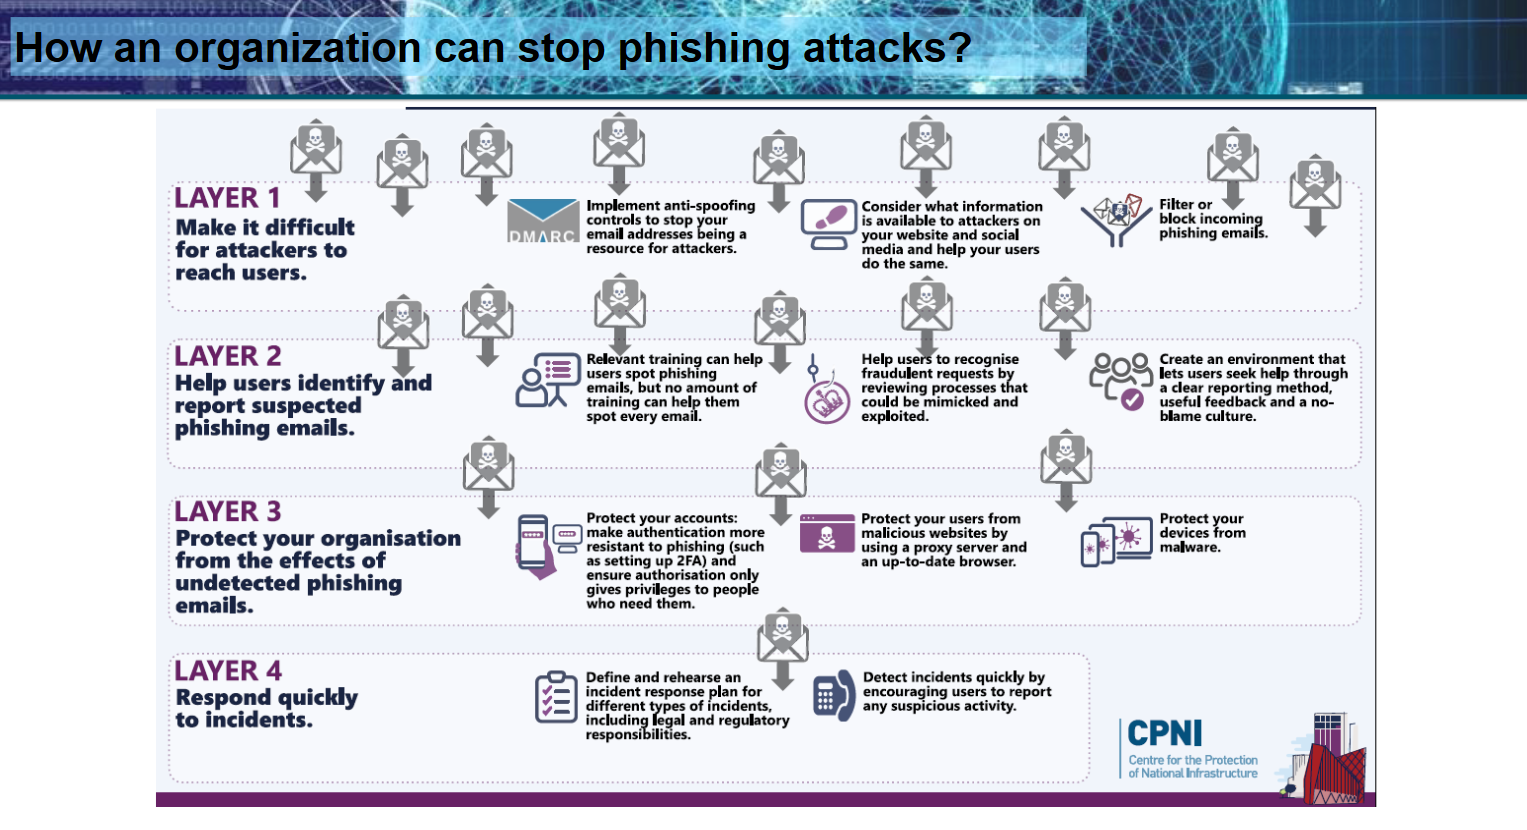
\includegraphics[width=1\textwidth]{images/5.png}
    \caption{Come fermare gli attacchi di phishing}
    \label{fig:my_label3}
\end{figure}